\section{Performance Evaluation}

There are some other proposed solutions in this field \citep{osvik,paladi,rudra2001efficient,matsui2006far,matsui2007power,konighofer2008fast,meushaw2005device}. We take some of the most prominent ones and compare it with our proposed solution.\\

\paragraph{Avoiding Memory Access}
Since the cache-timing attacks exploit the effect of memory access on the cache, any implementation that does not perform any table lookup won't suffer from this sort of attacks. But this solution has a major drawback. The performance is degraded by an order of magnitude. The SubBytes Transformation phase requires 16 table lookups for the 16 Bytes of a State matrix. The ShiftRows Transformation phase requires 16 shift operations. The MixColumns Transformation phase requires 8 shift operations, 8 conditional XOR operations and 12 mandatory XOR operations. Finally the AddRoundKey Transformation phase requires 16 XOR operations.\\

To summarize the fact, we need a total of 24 shift operations, 16 table lookups, 8 conditional XOR operations, 28 mandatory XOR operations for a single round. This is demonstrated in figure 10.

\begin{center}
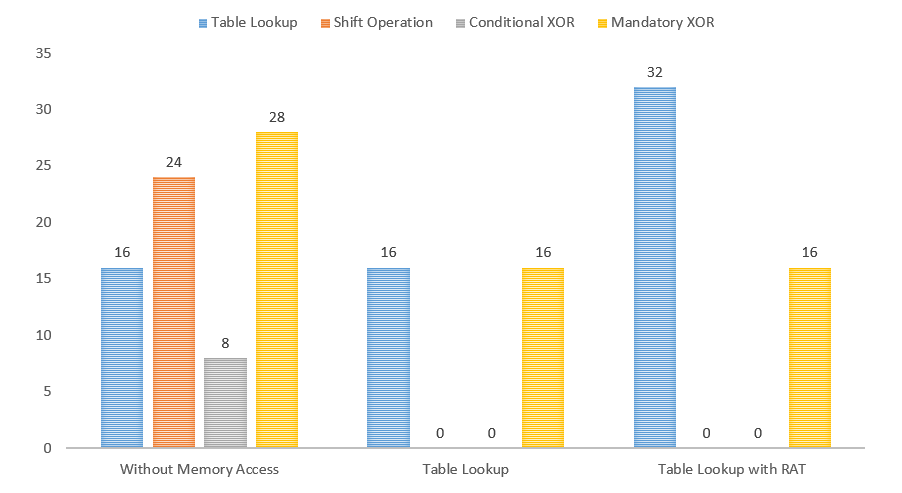
\includegraphics[scale=0.4,natwidth=902,natheight=493]{Figures/withnormal(new).png}
\captionof{figure}{Comparison of RAT with straightforward AES implementations in a single round. An implementation that completely avoids memory access requires 16 table lookups, 24 shift operations and 36 XOR operations (8 of which them are conditional), whereas introduction of RAT incurs 2 times more table lookups and 16 XOR operations in a single round.}
\label{fig: Comparison of RAT with Straightforward AES Implementation.}
\end{center}

In fact, the conditional XOR operation is vulnerable to timing attack too \citep{stallings5}. Other than lagging behind in terms of security, straightforward implementation required more computation time. So avoiding memory access doesn't save the day. But the positive side is, straightforward implementation doesn't need to maintain any sort of lookup table other than the S-Box. On the other hand table lookup with RAT has an overhead of maintaining two table. The Lookup table requires 4096 Bytes of memory space and RAT requires another 1024 Bytes of space.

\begin{center}
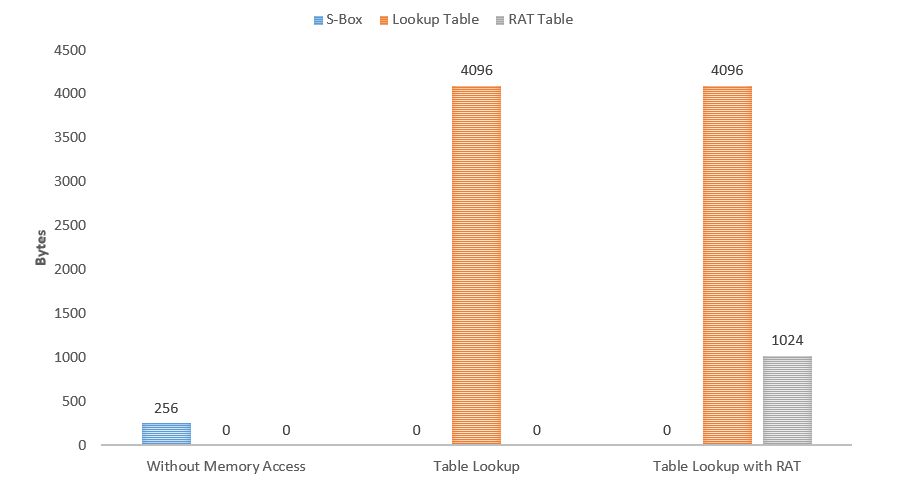
\includegraphics[scale=0.4,natwidth=902,natheight=493]{Figures/performance_memory(new).png}
\captionof{figure}{Performance Evaluation of RAT in terms of Memory Usage.}
\label{fig: Performance Evaluation of RAT in terms of Memory Usage.}
\end{center}

\paragraph{Disable Cache Sharing}
To protect against software-based attacks, it would suffice to prevent cache state effects from spanning process boundaries. But practically this is very expensive to achieve. On a single threaded processor, it would require flushing all caches during every context switch. On a processor with simultaneous multi threading, it would also require the logical processors to use separate logical caches, statically allocated within the physical cache; some modern processors do not support such a mode \citep{osvik}. Using RAT will not impose any restriction about cache sharing which is perfectly suitable for cloud environment and virtual machines (without causing evictions and filling).

\paragraph{Static or Disabled Cache}
One brutal countermeasure against the cache-base attacks is to completely disable the CPU's caching mechanism. Of course, the effect on performance would be devastating. A more attractive alternative is to activate a ``no-fill" mode where the memory accesses are serviced from the cache when they hit it, but accesses that miss the cache are serviced directly from the memory

\begin{enumerate}
\item Preload the AES tables into the cache
\item Activate the ``no-fill" mode
\item Perform encryption
\item Deactivating ``no-fill" mode
\end{enumerate}

The section spanning (1) and (2) is critical, and attacking process must not be allowed to run during this time \citep{osvik}. However, the major drawback of this approach is that, during the encryption process the overall system will be slowed down by a factor since cache access is limited during the encryption process. But using RAT, the ``no-fill" mode is not required. All the other processes can be allowed to access the cache even during the encryption proceeds.\\

\paragraph{Dynamic Table Storage}
The cache-based attacks observe memory access patterns to learn about the table lookups. Instead of eliminating these, we may try to decorrelate them. For example, one can use many copies of each table, placed at various offsets in memory, and have each table lookup use a pseudorandomly chosen table. Somewhat more compactly, one can use a single table, but pseudorandomly move it around memory several times during each encryption \citep{osvik}. But the major drawback of this approach is that, it will incur cache misses more than ever. This implies that the encryption process will be slowed down by a factor. More importantly the performance and security of this approach are very architecture dependent. Using RAT helps us alleviate this situation by obviating the need of moving around the Lookup table in the memory.

\subsection{Other Major Advantages}
Some important benefits of using the RAT are
\begin{itemize}
\item The Cipher Text remains the same and the AES implementation becomes a client dependent process. We don't need to worry about how other ends of the terminals are encrypting their data. As long as the key doesn't change, Cipher Text remains the same. 
\item No need of NOP operation. NOP operations are introduced to scramble uniform patterns in various fields. In case of cache-timing analysis, NOP operation would mean accessing Lookup table entry, but doing no operation with it.
\item No need to introduce disturbance in plaintext. Sometimes plaintext is modified before it is passed to the encrypting process. This sort of approach is not suitable for large scale application where the interface must be kept as simple as possible.

\end{itemize}
